\chapter{Approximation functions}

%%%%%%%%%%%%%%%%%%%%%%%%%%%%%%%%%%%%%%%%%%%%%%%%%%%%%%%%%%%%%%%%%%%%%%%%%%%%%%%%%%%%%%%%%%%%%%%%
%%%%%%%%%%%%%%%%%%%%%%%%%%%%%%%%%%%%%%%%%%%%%%%%%%%%%%%%%%%%%%%%%%%%%%%%%%%%%%%%%%%%%%%%%%%%%%%%
%%%%%%%%%%%%%%%%%%%%%%%%%%%%%%%%%%%%%%%%%%%%%%%%%%%%%%%%%%%%%%%%%%%%%%%%%%%%%%%%%%%%%%%%%%%%%%%%
%%%%%%%%%%%%%%%%%%%%%%%%%%%%%%%%%%%%%%%%%%%%%%%%%%%%%%%%%%%%%%%%%%%%%%%%%%%%%%%%%%%%%%%%%%%%%%%%
%%%%%%%%%%%%%%%%%%%%%%%%%%%%%%%%%%%%%%%%%%%%%%%%%%%%%%%%%%%%%%%%%%%%%%%%%%%%%%%%%%%%%%%%%%%%%%%%
%%%%%%%%%%%%%%%%%%%%%%%%%%%%%%%%%%%%%%%%%%%%%%%%%%%%%%%%%%%%%%%%%%%%%%%%%%%%%%%%%%%%%%%%%%%%%%%%
%%%%%%%%%%%%%%%%%%%%%%%%%%%%%%%%%%%%%%%%%%%%%%%%%%%%%%%%%%%%%%%%%%%%%%%%%%%%%%%%%%%%%%%%%%%%%%%%
%%%%%%%%%%%%%%%%%%%%%%%%%%%%%%%%%%%%%%%%%%%%%%%%%%%%%%%%%%%%%%%%%%%%%%%%%%%%%%%%%%%%%%%%%%%%%%%%
\section{Linear approximation functions defined on triangles}
\begin{eqnarray}
\label{bflintrn1}
N_1^{(1)} &=& \xi\ ,
\\
\label{bflintrn2}
N_2^{(1)} &=& \eta\ ,
\\
\label{bflintrn3}
N_3^{(1)} &=& 1 - \xi - \eta\ .
\end{eqnarray}
\begin{figure}
\begin{center}
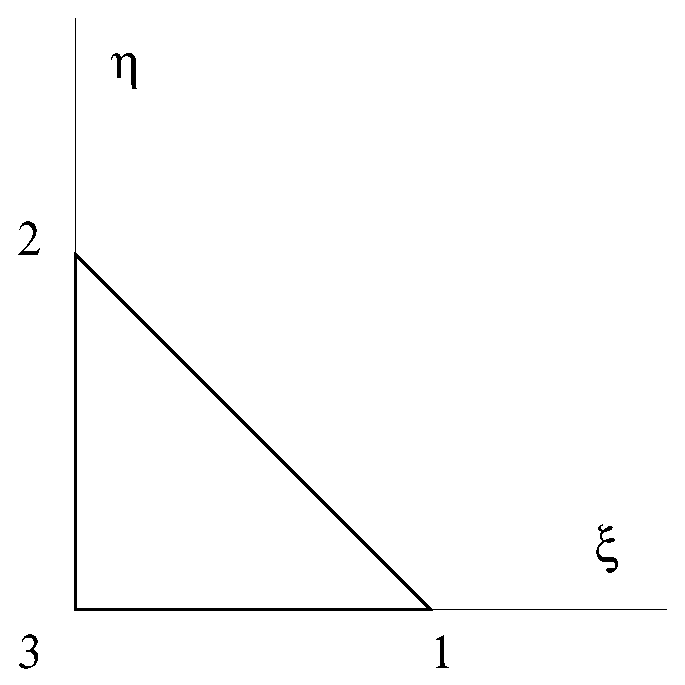
\includegraphics[width=80mm]{FIG/lintriang.eps}
\end{center}
\end{figure}
Partial derivatives with respect to $\xi$ have form
\begin{eqnarray}
\label{bflintrdx1}
\ppd{N_1^{(1)}}{\xi} &=& 1\ ,
\\
\label{bflintrdx2}
\ppd{N_2^{(1)}}{\xi} &=& 0\ ,
\\
\label{bflintrdx3}
\ppd{N_3^{(1)}}{\xi} &=& - 1\ .
\end{eqnarray}
Partial derivatives with respect to $\eta$ have form
\begin{eqnarray}
\label{bflintrdy1}
\ppd{N_1^{(1)}}{\eta} &=& 0\ ,
\\
\label{bflintrdy2}
\ppd{N_2^{(1)}}{\eta} &=& 1\ ,
\\
\label{bflintrdy3}
\ppd{N_3^{(1)}}{\eta} &=& - 1\ .
\end{eqnarray}


%%%%%%%%%%%%%%%%%%%%%%%%%%%%%%%%%%%%%%%%%%%%%%%%%%%%%%%%%%%%%%%%%%%%%%%%%%%%%%%%%%%%%%%%%%%%%%%%
%%%%%%%%%%%%%%%%%%%%%%%%%%%%%%%%%%%%%%%%%%%%%%%%%%%%%%%%%%%%%%%%%%%%%%%%%%%%%%%%%%%%%%%%%%%%%%%%
%%%%%%%%%%%%%%%%%%%%%%%%%%%%%%%%%%%%%%%%%%%%%%%%%%%%%%%%%%%%%%%%%%%%%%%%%%%%%%%%%%%%%%%%%%%%%%%%
%%%%%%%%%%%%%%%%%%%%%%%%%%%%%%%%%%%%%%%%%%%%%%%%%%%%%%%%%%%%%%%%%%%%%%%%%%%%%%%%%%%%%%%%%%%%%%%%
\section{Quadratic approximation functions defined on triangles}
\begin{eqnarray}
\label{bfquadtrn1}
N_1^{(2)} &=& 2\xi(\xi-0.5)\ ,
\\
\label{bfquadtrn2}
N_2^{(2)} &=& 2\eta(\eta-0.5)\ ,
\\
\label{bfquadtrn3}
N_3^{(2)} &=& 2(1 - \xi - \eta)(0.5-\xi-\eta)\ .
\\
\label{bfquadtrn4}
N_4^{(2)} &=& 4 \xi \eta \ ,
\\
\label{bfquadtrn5}
N_5^{(2)} &=& 4 \eta (1 - \xi - \eta)\ ,
\\
\label{bfquadtrn6}
N_6^{(2)} &=& 4 \xi (1 - \xi - \eta)\ ,
\\
\end{eqnarray}
\begin{figure}
\begin{center}
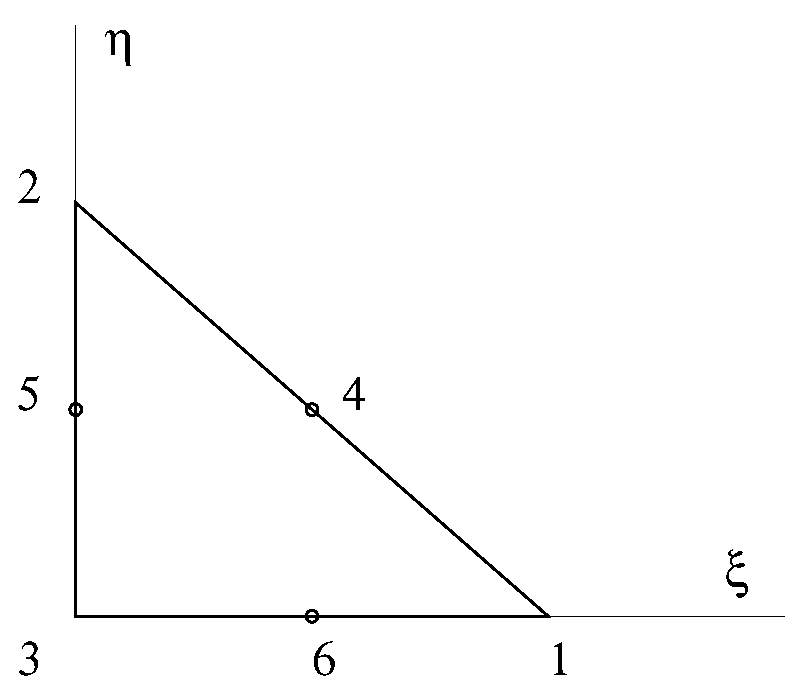
\includegraphics[width=80mm]{FIG/quadtriang.eps}
\end{center}
\end{figure}
Partial derivatives with respect to $\xi$ have form
\begin{eqnarray}
\label{bfquadtrdx1}
\ppd{N_1^{(2)}}{\xi} &=& 4 \xi - 1\ ,
\\
\label{bfquadtrdx2}
\ppd{N_2^{(2)}}{\xi} &=& 0\ ,
\\
\label{bfquadtrdx3}
\ppd{N_3^{(2)}}{\xi} &=& 4 \xi + 4 \eta - 3\ ,
\\
\label{bfquadtrdx4}
\ppd{N_4^{(2)}}{\xi} &=& 4 \eta\ ,
\\
\label{bfquadtrdx5}
\ppd{N_5^{(2)}}{\xi} &=& -4 \eta\ ,
\\
\label{bfquadtrdx6}
\ppd{N_6^{(2)}}{\xi} &=& 4 - 8 \xi - 4 \eta\ .
\end{eqnarray}
Partial derivatives with respect to $\eta$ have form
\begin{eqnarray}
\label{bfquadtrdy1}
\ppd{N_1^{(2)}}{\eta} &=& 0\ ,
\\
\label{bfquadtrdy2}
\ppd{N_2^{(2)}}{\eta} &=& 4 \eta -1\ ,
\\
\label{bfquadtrdy3}
\ppd{N_3^{(2)}}{\eta} &=& 4 \xi + 4 \eta -3\ ,
\\
\label{bfquadtrdy4}
\ppd{N_4^{(2)}}{\eta} &=& 4 \xi\ ,
\\
\label{bfquadtrdy5}
\ppd{N_5^{(2)}}{\eta} &=& 4 - 4 \xi - 8 \eta\ ,
\\
\label{bfquadtrdy6}
\ppd{N_6^{(2)}}{\eta} &=& - 4 \xi\ .
\end{eqnarray}



%%%%%%%%%%%%%%%%%%%%%%%%%%%%%%%%%%%%%%%%%%%%%%%%%%%%%%%%%%%%%%%%%%%%%%%%%%%%%%%%%%%%%%%%%%%%%%%%
%%%%%%%%%%%%%%%%%%%%%%%%%%%%%%%%%%%%%%%%%%%%%%%%%%%%%%%%%%%%%%%%%%%%%%%%%%%%%%%%%%%%%%%%%%%%%%%%
%%%%%%%%%%%%%%%%%%%%%%%%%%%%%%%%%%%%%%%%%%%%%%%%%%%%%%%%%%%%%%%%%%%%%%%%%%%%%%%%%%%%%%%%%%%%%%%%
%%%%%%%%%%%%%%%%%%%%%%%%%%%%%%%%%%%%%%%%%%%%%%%%%%%%%%%%%%%%%%%%%%%%%%%%%%%%%%%%%%%%%%%%%%%%%%%%
\section{Bi-linear approximation functions defined on quadrilateral elements}
$\xi$ and $\eta$ are natural coordinates defined on square $\langle-1;1\rangle\times\langle-1;1\rangle$. The functions
have form
\begin{eqnarray}
\label{bflinquadn1}
N_1^{(1)} &=& \del{1}{4} (1 + \xi) (1 + \eta)\ ,
\\
\label{bflinquadn2}
N_2^{(1)} &=& \del{1}{4} (1 - \xi) (1 + \eta)\ ,
\\
\label{bflinquadn3}
N_3^{(1)} &=& \del{1}{4} (1 - \xi) (1 - \eta)\ ,
\\
\label{bflinquadn4}
N_4^{(1)} &=& \del{1}{4} (1 + \xi) (1 - \eta)\ .
\end{eqnarray}
\begin{figure}
\begin{center}
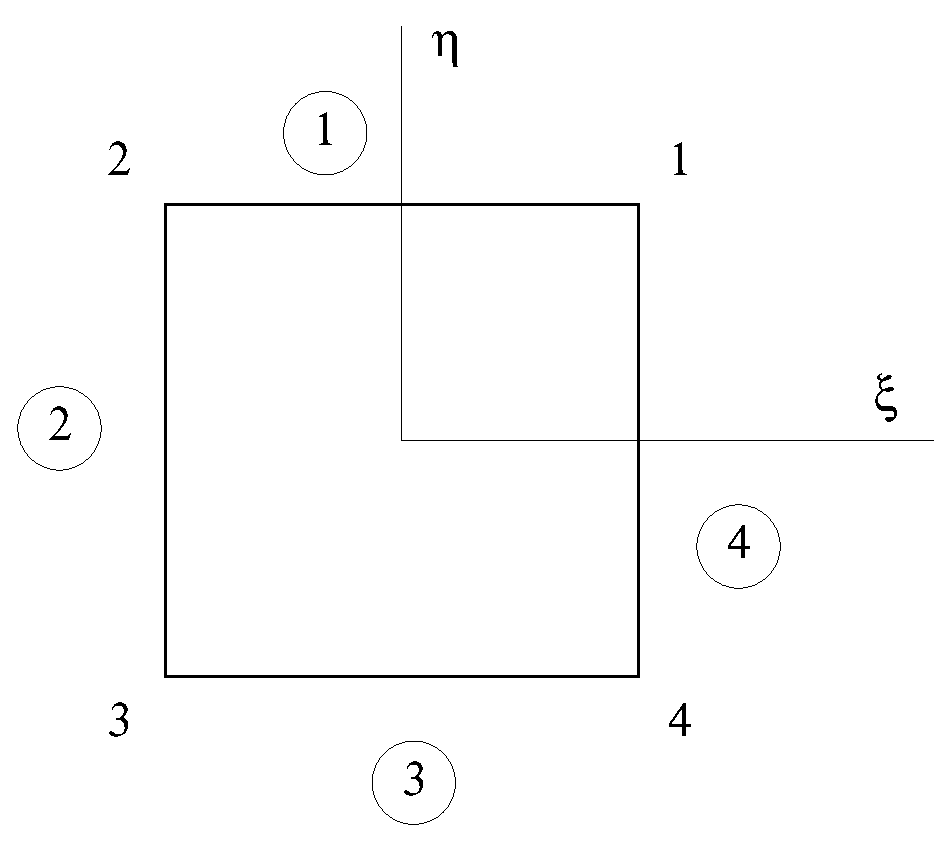
\includegraphics[width=80mm]{FIG/linquad.eps}
\end{center}
\end{figure}
Partial derivatives with respect to $\xi$ have form
\begin{eqnarray}
\label{bflinquaddx1}
\ppd{N_1^{(1)}}{\xi} &=& \del{1}{4} (1 + \eta)\ ,
\\
\label{bflinquaddx2}
\ppd{N_2^{(1)}}{\xi} &=& - \del{1}{4} (1 + \eta)\ ,
\\
\label{bflinquaddx3}
\ppd{N_3^{(1)}}{\xi} &=& - \del{1}{4} (1 - \eta)\ ,
\\
\label{bflinquaddx4}
\ppd{N_4^{(1)}}{\xi} &=& \del{1}{4} (1 - \eta)\ .
\end{eqnarray}
Partial derivatives with respect to $\eta$ have form
\begin{eqnarray}
\label{bflinquaddy1}
\ppd{N_1^{(1)}}{\eta} &=& \del{1}{4} (1 + \xi)\ ,
\\
\label{bflinquaddy2}
\ppd{N_2^{(1)}}{\eta} &=& \del{1}{4} (1 - \xi)\ ,
\\
\label{bflinquaddy3}
\ppd{N_3^{(1)}}{\eta} &=& - \del{1}{4} (1 - \xi)\ ,
\\
\label{bflinquaddy4}
\ppd{N_4^{(1)}}{\eta} &=& - \del{1}{4} (1 + \xi)\ .
\end{eqnarray}

%%%%%%%%%%%%%%%%%%%%%%%%%%%%%%%%%%%%%%%%%%%%%%%%%%%%%%%%%%%%%%%%%%%%%%%%%%%%%%%%%%%%%%%%%%%%%%%%
%%%%%%%%%%%%%%%%%%%%%%%%%%%%%%%%%%%%%%%%%%%%%%%%%%%%%%%%%%%%%%%%%%%%%%%%%%%%%%%%%%%%%%%%%%%%%%%%
%%%%%%%%%%%%%%%%%%%%%%%%%%%%%%%%%%%%%%%%%%%%%%%%%%%%%%%%%%%%%%%%%%%%%%%%%%%%%%%%%%%%%%%%%%%%%%%%
%%%%%%%%%%%%%%%%%%%%%%%%%%%%%%%%%%%%%%%%%%%%%%%%%%%%%%%%%%%%%%%%%%%%%%%%%%%%%%%%%%%%%%%%%%%%%%%%
\section{Bi-quadratic approximation functions defined on quadrilateral elements}
$\xi$ and $\eta$ are natural coordinates defined on square $\langle-1;1\rangle\times\langle-1;1\rangle$. The functions
have form
\begin{eqnarray}
\label{bfquadquadn1}
N_1^{(2)} &=& \del{1}{4} (1 + \xi) (1 + \eta) (\xi + \eta - 1)\ ,
\\
\label{bfquadquadn2}
N_2^{(2)} &=& \del{1}{4} (1 - \xi) (1 + \eta) (- \xi + \eta - 1)\ ,
\\
\label{bfquadquadn3}
N_3^{(2)} &=& \del{1}{4} (1 - \xi) (1 - \eta) (- \xi - \eta - 1)\ ,
\\
\label{bfquadquadn4}
N_4^{(2)} &=& \del{1}{4} (1 + \xi) (1 - \eta) (\xi - \eta - 1)\ ,
\\
\label{bfquadquadn5}
N_5^{(2)} &=& \del{1}{2} (1 - \xi^2) (1 + \eta)\ ,
\\
\label{bfquadquadn6}
N_6^{(2)} &=& \del{1}{2} (1 - \xi) (1 - \eta^2)\ ,
\\
\label{bfquadquadn7}
N_7^{(2)} &=& \del{1}{2} (1 - \xi^2) (1 - \eta)\ ,
\\
\label{bfquadquadn8}
N_8^{(2)} &=& \del{1}{2} (1 + \xi) (1 - \eta^2)\ .
\end{eqnarray}
\begin{figure}
\begin{center}
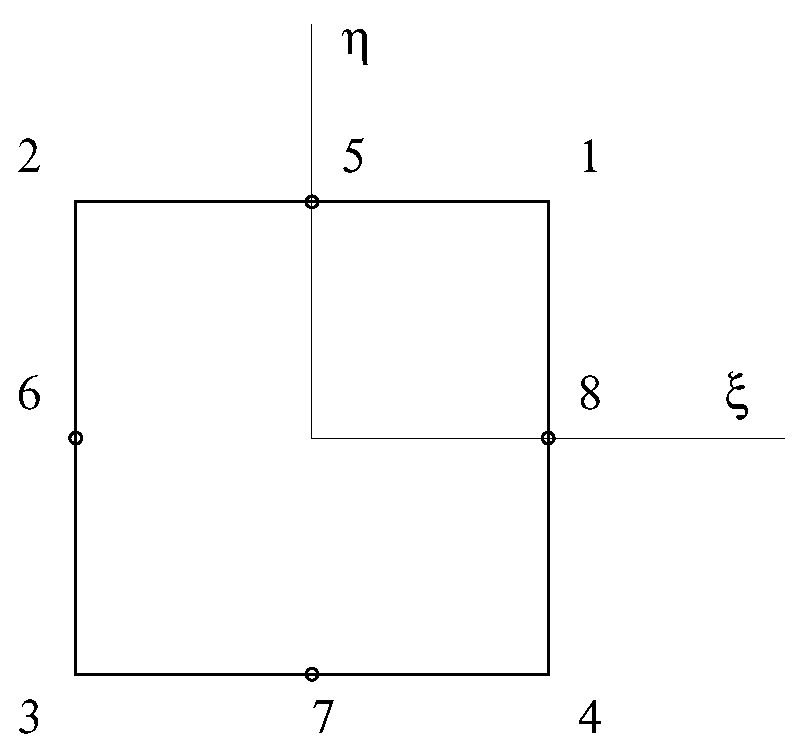
\includegraphics[width=80mm]{FIG/quadquad.eps}
\end{center}
\end{figure}
Partial derivatives with respect to $\xi$ have form
\begin{eqnarray}
\label{bfquadquaddx1}
\ppd{N_1^{(2)}}{\xi} &=& \del{1}{4} (1 + \eta) (\xi + \eta - 1) +
\del{1}{4} (1 + \xi) (1 + \eta)\ ,
\\
\label{bfquadquaddx2}
\ppd{N_2^{(2)}}{\xi} &=& - \del{1}{4} (1 + \eta) (- \xi + \eta - 1) -
\del{1}{4} (1 - \xi) (1 + \eta)\ ,
\\
\label{bfquadquaddx3}
\ppd{N_3^{(2)}}{\xi} &=& - \del{1}{4} (1 - \eta) (- \xi - \eta - 1) -
\del{1}{4} (1 - \xi) (1 - \eta)\ ,
\\
\label{bfquadquaddx4}
\ppd{N_4^{(2)}}{\xi} &=& \del{1}{4} (1 - \eta) (\xi - \eta - 1) +
\del{1}{4} (1 + \xi) (1 - \eta)\ ,
\\
\label{bfquadquaddx5}
\ppd{N_5^{(2)}}{\xi} &=& - \xi (1 + \eta)\ ,
\\
\label{bfquadquaddx6}
\ppd{N_6^{(2)}}{\xi} &=& - \del{1}{2} (1 - \eta^2)\ ,
\\
\label{bfquadquaddx7}
\ppd{N_7^{(2)}}{\xi} &=& - \xi (1 - \eta)\ ,
\\
\label{bfquadquaddx8}
\ppd{N_8^{(2)}}{\xi} &=& \del{1}{2} (1 - \eta^2)\ .
\end{eqnarray}
Partial derivatives with respect to $\eta$ have form
\begin{eqnarray}
\label{bfquadquaddy1}
\ppd{N_1^{(2)}}{\eta} &=& \del{1}{4} (1 + \xi) (\xi + \eta - 1) +
\del{1}{4} (1 + \xi) (1 + \eta)\ ,
\\
\label{bfquadquaddy2}
\ppd{N_2^{(2)}}{\eta} &=& \del{1}{4} (1 - \xi) (- \xi + \eta - 1) +
\del{1}{4} (1 - \xi) (1 + \eta)\ ,
\\
\label{bfquadquaddy3}
\ppd{N_3^{(2)}}{\eta} &=& - \del{1}{4} (1 - \xi) (- \xi - \eta - 1) -
\del{1}{4} (1 - \xi) (1 - \eta)\ ,
\\
\label{bfquadquaddy4}
\ppd{N_4^{(2)}}{\eta} &=& - \del{1}{4} (1 + \xi) (\xi - \eta - 1) -
\del{1}{4} (1 + \xi) (1 - \eta)\ ,
\\
\label{bfquadquaddy5}
\ppd{N_5^{(2)}}{\eta} &=& \del{1}{2} (1 - \xi^2)\ ,
\\
\label{bfquadquaddy6}
\ppd{N_6^{(2)}}{\eta} &=& (1 - \xi) (- \eta)\ ,
\\
\label{bfquadquaddy7}
\ppd{N_7^{(2)}}{\eta} &=& - \del{1}{2} (1 - \xi^2)\ ,
\\
\label{bfquadquaddy8}
\ppd{N_8^{(2)}}{\eta} &=& (1 + \xi) (- \eta)\ .
\end{eqnarray}

%%%%%%%%%%%%%%%%%%%%%%%%%%%%%%%%%%%%%%%%%%%%%%%%%%%%%%%%%%%%%%%%%%%%%%%%%%%%%
%%%%%%%%%%%%%%%%%%%%%%%%%%%%%%%%%%%%%%%%%%%%%%%%%%%%%%%%%%%%%%%%%%%%%%%%%%%%%%%%%%%%%%%%%%%%%%%%
%%%%%%%%%%%%%%%%%%%%%%%%%%%%%%%%%%%%%%%%%%%%%%%%%%%%%%%%%%%%%%%%%%%%%%%%%%%%%%%%%%%%%%%%%%%%%%%%
%%%%%%%%%%%%%%%%%%%%%%%%%%%%%%%%%%%%%%%%%%%%%%%%%%%%%%%%%%%%%%%%%%%%%%%%%%%%%%%%%%%%%%%%%%%%%%%%
%%%%%%%%%%%%%%%%%%%%%%%%%%%%%%%%%%%%%%%%%%%%%%%%%%%%%%%%%%%%%%%%%%%%%%%%%%%%%%%%%%%%%%%%%%%%%%%%
\section{Tri-linear approximation functions defined on hexahedral elements}
$\xi$, $\eta$ and $\zeta$ are natural coordinates defined on cube
$\langle-1;1\rangle\times\langle-1;1\rangle\times\langle-1;1\rangle$. The functions have form
\begin{eqnarray}
\label{bflinhexn1}
N_1^{(1)} &=& \del{1}{8} (1 + \xi) (1 + \eta) (1 + \zeta)\ ,
\\
\label{bflinhexn2}
N_2^{(1)} &=& \del{1}{8} (1 - \xi) (1 + \eta) (1 + \zeta)\ ,
\\
\label{bflinhexn3}
N_3^{(1)} &=& \del{1}{8} (1 - \xi) (1 - \eta) (1 + \zeta)\ ,
\\
\label{bflinhexn4}
N_4^{(1)} &=& \del{1}{8} (1 + \xi) (1 - \eta) (1 + \zeta)\ ,
\\
\label{bflinhexn5}
N_5^{(1)} &=& \del{1}{8} (1 + \xi) (1 + \eta) (1 - \zeta)\ ,
\\
\label{bflinhexn6}
N_6^{(1)} &=& \del{1}{8} (1 - \xi) (1 + \eta) (1 - \zeta)\ ,
\\
\label{bflinhexn7}
N_7^{(1)} &=& \del{1}{8} (1 - \xi) (1 - \eta) (1 - \zeta)\ ,
\\
\label{bflinhexn8}
N_8^{(1)} &=& \del{1}{8} (1 + \xi) (1 - \eta) (1 - \zeta)\ .
\end{eqnarray}
\begin{figure}
\begin{center}
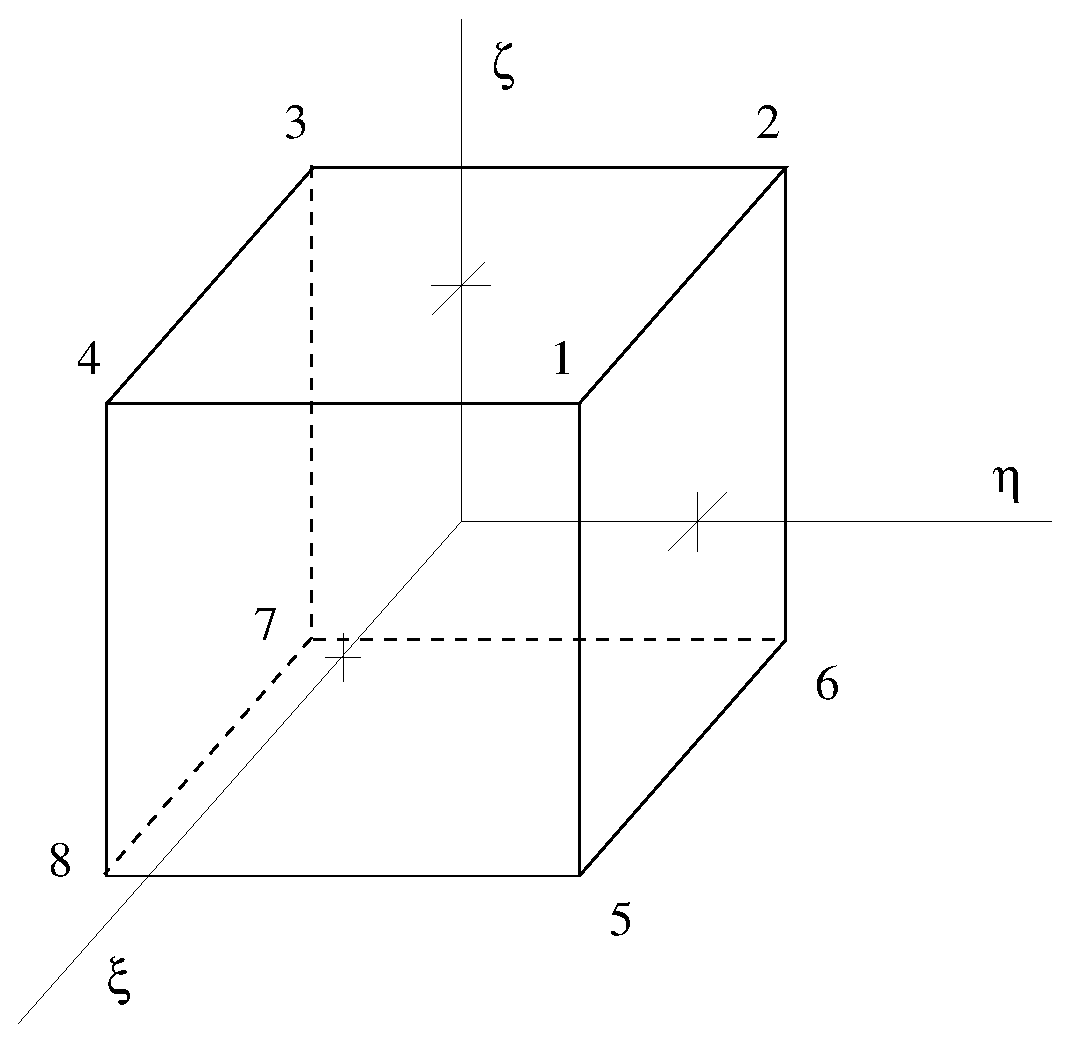
\includegraphics[width=80mm]{FIG/linhex.eps}
\end{center}
\end{figure}
Partial derivatives with respect to $\xi$ have form
\begin{eqnarray}
\label{bflinhexdx1}
\ppd{N_1^{(1)}}{\xi} &=& \del{1}{8} (1 + \eta) (1 + \zeta)\ ,
\\
\label{bflinhexdx2}
\ppd{N_2^{(1)}}{\xi} &=& - \del{1}{8} (1 + \eta) (1 + \zeta)\ ,
\\
\label{bflinhexdx3}
\ppd{N_3^{(1)}}{\xi} &=& - \del{1}{8} (1 - \eta) (1 + \zeta)\ ,
\\
\label{bflinhexdx4}
\ppd{N_4^{(1)}}{\xi} &=& \del{1}{8} (1 - \eta) (1 + \zeta)\ ,
\\
\label{bflinhexdx5}
\ppd{N_5^{(1)}}{\xi} &=& \del{1}{8} (1 + \eta) (1 - \zeta)\ ,
\\
\label{bflinhexdx6}
\ppd{N_6^{(1)}}{\xi} &=& - \del{1}{8} (1 + \eta) (1 - \zeta)\ ,
\\
\label{bflinhexdx7}
\ppd{N_7^{(1)}}{\xi} &=& - \del{1}{8} (1 - \eta) (1 - \zeta)\ ,
\\
\label{bflinhexdx8}
\ppd{N_8^{(1)}}{\xi} &=& \del{1}{8} (1 - \eta) (1 - \zeta)\ .
\end{eqnarray}
Partial derivatives with respect to $\eta$ have form
\begin{eqnarray}
\label{bflinhexdy1}
\ppd{N_1^{(1)}}{\eta} &=& \del{1}{8} (1 + \xi) (1 + \zeta)\ ,
\\
\label{bflinhexdy2}
\ppd{N_2^{(1)}}{\eta} &=& \del{1}{8} (1 - \xi) (1 + \zeta)\ ,
\\
\label{bflinhexdy3}
\ppd{N_3^{(1)}}{\eta} &=& - \del{1}{8} (1 - \xi) (1 + \zeta)\ ,
\\
\label{bflinhexdy4}
\ppd{N_4^{(1)}}{\eta} &=& - \del{1}{8} (1 + \xi) (1 + \zeta)\ ,
\\
\label{bflinhexdy5}
\ppd{N_5^{(1)}}{\eta} &=& \del{1}{8} (1 + \xi) (1 - \zeta)\ ,
\\
\label{bflinhexdy6}
\ppd{N_6^{(1)}}{\eta} &=& \del{1}{8} (1 - \xi) (1 - \zeta)\ ,
\\
\label{bflinhexdy7}
\ppd{N_7^{(1)}}{\eta} &=& - \del{1}{8} (1 - \xi) (1 - \zeta)\ ,
\\
\label{bflinhexdy8}
\ppd{N_8^{(1)}}{\eta} &=& - \del{1}{8} (1 + \xi) (1 - \zeta)\ .
\end{eqnarray}
Partial derivatives with respect to $\zeta$ have form
\begin{eqnarray}
\label{bflinhexdz1}
\ppd{N_1^{(1)}}{\zeta} &=& \del{1}{8} (1 + \xi) (1 + \eta)\ ,
\\
\label{bflinhexdz2}
\ppd{N_2^{(1)}}{\zeta} &=& \del{1}{8} (1 - \xi) (1 + \eta)\ ,
\\
\label{bflinhexdz3}
\ppd{N_3^{(1)}}{\zeta} &=& \del{1}{8} (1 - \xi) (1 - \eta)\ ,
\\
\label{bflinhexdz4}
\ppd{N_4^{(1)}}{\zeta} &=& \del{1}{8} (1 + \xi) (1 - \eta)\ ,
\\
\label{bflinhexdz5}
\ppd{N_5^{(1)}}{\zeta} &=& - \del{1}{8} (1 + \xi) (1 + \eta)\ ,
\\
\label{bflinhexdz6}
\ppd{N_6^{(1)}}{\zeta} &=& - \del{1}{8} (1 - \xi) (1 + \eta)\ ,
\\
\label{bflinhexdz7}
\ppd{N_7^{(1)}}{\zeta} &=& - \del{1}{8} (1 - \xi) (1 - \eta)\ ,
\\
\label{bflinhexdz8}
\ppd{N_8^{(1)}}{\zeta} &=& - \del{1}{8} (1 + \xi) (1 - \eta)\ .
\end{eqnarray}



%%%%%%%%%%%%%%%%%%%%%%%%%%%%%%%%%%%%%%%%%%%%%%%%%%%%%%%%%%%%%%%%%%%%%%%%%%%%%%%%%%%%%%%%%%%%%%%%
%%%%%%%%%%%%%%%%%%%%%%%%%%%%%%%%%%%%%%%%%%%%%%%%%%%%%%%%%%%%%%%%%%%%%%%%%%%%%%%%%%%%%%%%%%%%%%%%
%%%%%%%%%%%%%%%%%%%%%%%%%%%%%%%%%%%%%%%%%%%%%%%%%%%%%%%%%%%%%%%%%%%%%%%%%%%%%%%%%%%%%%%%%%%%%%%%
%%%%%%%%%%%%%%%%%%%%%%%%%%%%%%%%%%%%%%%%%%%%%%%%%%%%%%%%%%%%%%%%%%%%%%%%%%%%%%%%%%%%%%%%%%%%%%%%
\section{Tri-quadratic approximation functions defined on hexahedral elements}
$\xi$, $\eta$ and $\zeta$ are natural coordinates defined on cube
$\langle-1;1\rangle\times\langle-1;1\rangle\times\langle-1;1\rangle$. The functions have form
\begin{eqnarray}
\label{bfquadhexn1}
N_{1}^{(2)} &=& \del{1}{8} (1 + \xi) (1 + \eta) (1 + \zeta)
(\xi + \eta + \zeta - 2)\ ,
\\ \label{bfquadhexn2}
N_{2}^{(2)} &=& \del{1}{8} (1 - \xi) (1 + \eta) (1 + \zeta)
(- \xi + \eta + \zeta - 2)\ ,
\\ \label{bfquadhexn3}
N_{3}^{(2)} &=& \del{1}{8} (1 - \xi) (1 - \eta) (1 + \zeta)
(- \xi - \eta + \zeta - 2)\ ,
\\ \label{bfquadhexn4}
N_{4}^{(2)} &=& \del{1}{8} (1 + \xi) (1 - \eta) (1 + \zeta)
(\xi - \eta + \zeta - 2)\ ,
\\ \label{bfquadhexn5}
N_{5}^{(2)} &=& \del{1}{8} (1 + \xi) (1 + \eta) (1 - \zeta)
(\xi + \eta - \zeta - 2)\ ,
\\ \label{bfquadhexn6}
N_{6}^{(2)} &=& \del{1}{8} (1 - \xi) (1 + \eta) (1 - \zeta)
(- \xi + \eta - \zeta - 2)\ ,
\\ \label{bfquadhexn7}
N_{7}^{(2)} &=& \del{1}{8} (1 - \xi) (1 - \eta) (1 - \zeta)
(- \xi - \eta - \zeta - 2)\ ,
\\ \label{bfquadhexn8}
N_{8}^{(2)} &=& \del{1}{8} (1 + \xi) (1 - \eta) (1 - \zeta)
(\xi - \eta - \zeta - 2)\ ,
\\ \label{bfquadhexn9}
N_{9}^{(2)} &=& \del{1}{4} (1 - \xi^2) (1 + \eta) (1 + \zeta)\ ,
\\ \label{bfquadhexn10}
N_{10}^{(2)} &=& \del{1}{4} (1 - \xi) (1 - \eta^2) (1 + \zeta)\ ,
\\ \label{bfquadhexn11}
N_{11}^{(2)} &=& \del{1}{4} (1 - \xi^2) (1 - \eta) (1 + \zeta)\ ,
\\ \label{bfquadhexn12}
N_{12}^{(2)} &=& \del{1}{4} (1 + \xi) (1 - \eta^2) (1 + \zeta)\ ,
\\ \label{bfquadhexn13}
N_{13}^{(2)} &=& \del{1}{4} (1 + \xi) (1 + \eta) (1 - \zeta^2)\ ,
\\ \label{bfquadhexn14}
N_{14}^{(2)} &=& \del{1}{4} (1 - \xi) (1 + \eta) (1 - \zeta^2)\ ,
\\ \label{bfquadhexn15}
N_{15}^{(2)} &=& \del{1}{4} (1 - \xi) (1 - \eta) (1 - \zeta^2)\ ,
\\ \label{bfquadhexn16}
N_{16}^{(2)} &=& \del{1}{4} (1 + \xi) (1 - \eta) (1 - \zeta^2)\ ,
\\ \label{bfquadhexn17}
N_{17}^{(2)} &=& \del{1}{4} (1 - \xi^2) (1 + \eta) (1 - \zeta)\ ,
\\ \label{bfquadhexn18}
N_{18}^{(2)} &=& \del{1}{4} (1 - \xi) (1 - \eta^2) (1 - \zeta)\ ,
\\ \label{bfquadhexn19}
N_{19}^{(2)} &=& \del{1}{4} (1 - \xi^2) (1 - \eta) (1 - \zeta)\ ,
\\ \label{bfquadhexn20}
N_{20}^{(2)} &=& \del{1}{4} (1 + \xi) (1 - \eta^2) (1 - \zeta)\ .
\end{eqnarray}
\begin{figure}
\begin{center}
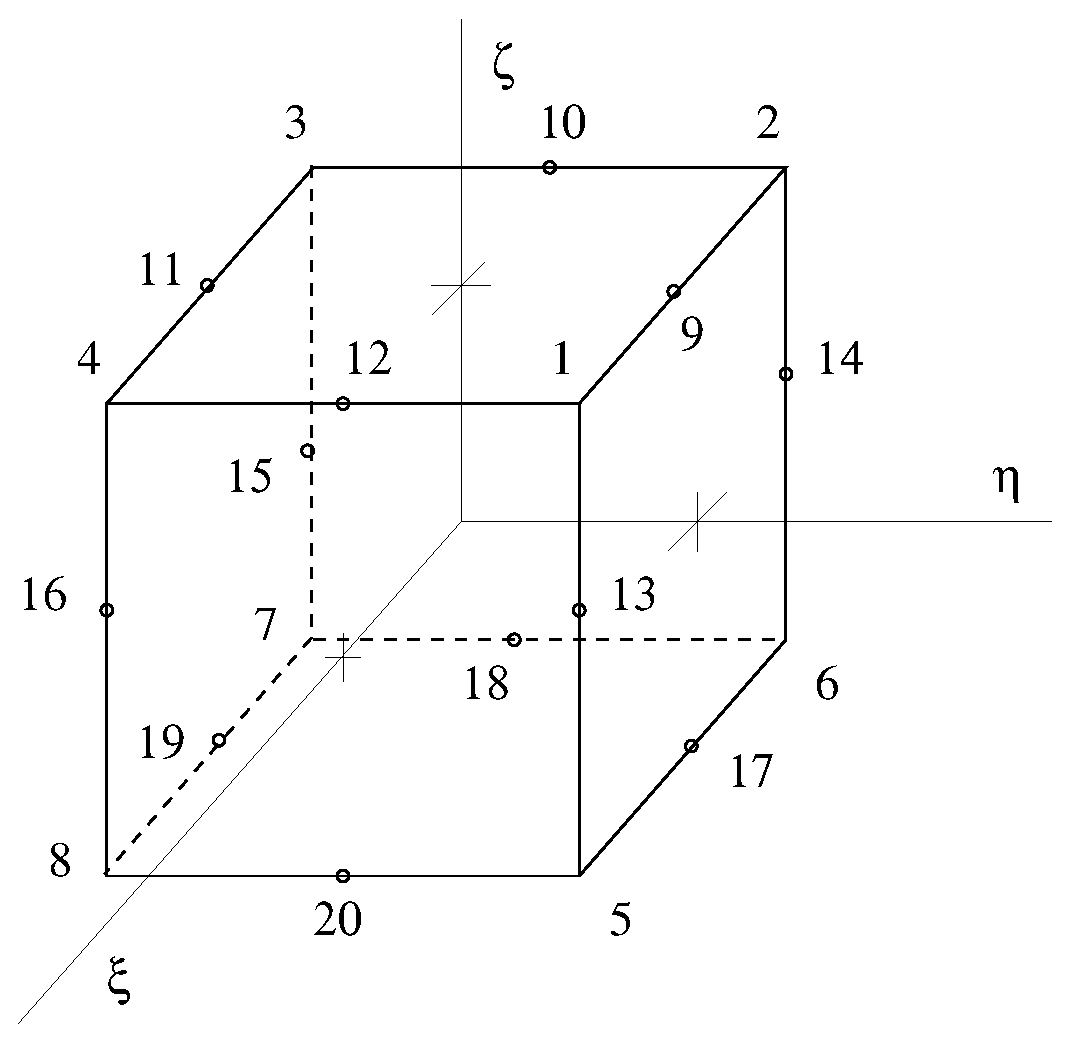
\includegraphics[width=80mm]{FIG/quadhex.eps}
\end{center}
\end{figure}
Partial derivatives with respect to $\xi$ have form
\begin{eqnarray}
\label{bfquadhexdx1}
\ppd{N_{1}^{(2)}}{\xi} &=& \del{1}{8} (1 + \eta) (1 + \zeta)
(\xi + \eta + \zeta - 2) + \del{1}{8} (1 + \xi) (1 + \eta) (1 + \zeta)\ ,
\\ \label{bfquadhexdx2}
\ppd{N_{2}^{(2)}}{\xi} &=& - \del{1}{8} (1 + \eta) (1 + \zeta)
(- \xi + \eta + \zeta - 2) - \del{1}{8} (1 - \xi) (1 + \eta) (1 + \zeta)\ ,
\\ \label{bfquadhexdx3}
\ppd{N_{3}^{(2)}}{\xi} &=& - \del{1}{8} (1 - \eta) (1 + \zeta)
(- \xi - \eta + \zeta - 2) - \del{1}{8} (1 - \xi) (1 - \eta) (1 + \zeta)\ ,
\\ \label{bfquadhexdx4}
\ppd{N_{4}^{(2)}}{\xi} &=& \del{1}{8} (1 - \eta) (1 + \zeta)
(\xi - \eta + \zeta - 2) + \del{1}{8} (1 + \xi) (1 - \eta) (1 + \zeta)\ ,
\\ \label{bfquadhexdx5}
\ppd{N_{5}^{(2)}}{\xi} &=& \del{1}{8} (1 + \eta) (1 - \zeta)
(\xi + \eta - \zeta - 2) + \del{1}{8} (1 + \xi) (1 + \eta) (1 - \zeta)\ ,
\\ \label{bfquadhexdx6}
\ppd{N_{6}^{(2)}}{\xi} &=& - \del{1}{8} (1 + \eta) (1 - \zeta)
(- \xi + \eta - \zeta - 2) - \del{1}{8} (1 - \xi) (1 + \eta) (1 - \zeta)\ ,
\\ \label{bfquadhexdx7}
\ppd{N_{7}^{(2)}}{\xi} &=& - \del{1}{8} (1 - \eta) (1 - \zeta)
(- \xi - \eta - \zeta - 2) - \del{1}{8} (1 - \xi) (1 - \eta) (1 - \zeta)\ ,
\\ \label{bfquadhexdx8}
\ppd{N_{8}^{(2)}}{\xi} &=& \del{1}{8} (1 - \eta) (1 - \zeta)
(\xi - \eta - \zeta - 2) + \del{1}{8} (1 + \xi) (1 - \eta) (1 - \zeta)\ ,
\\ \label{bfquadhexdx9}
\ppd{N_{9}^{(2)}}{\xi} &=& - \del{1}{2} \xi (1 + \eta) (1 + \zeta)\ ,
\\ \label{bfquadhexdx10}
\ppd{N_{10}^{(2)}}{\xi} &=& - \del{1}{4} (1 - \eta^2) (1 + \zeta)\ ,
\\ \label{bfquadhexdx11}
\ppd{N_{11}^{(2)}}{\xi} &=& - \del{1}{2} \xi (1 - \eta) (1 + \zeta)\ ,
\\ \label{bfquadhexdx12}
\ppd{N_{12}^{(2)}}{\xi} &=& \del{1}{4} (1 - \eta^2) (1 + \zeta)\ ,
\\ \label{bfquadhexdx13}
\ppd{N_{13}^{(2)}}{\xi} &=& \del{1}{4} (1 + \eta) (1 - \zeta^2)\ ,
\\ \label{bfquadhexdx14}
\ppd{N_{14}^{(2)}}{\xi} &=& - \del{1}{4} (1 + \eta) (1 - \zeta^2)\ ,
\\ \label{bfquadhexdx15}
\ppd{N_{15}^{(2)}}{\xi} &=& - \del{1}{4} (1 - \eta) (1 - \zeta^2)\ ,
\\ \label{bfquadhexdx16}
\ppd{N_{16}^{(2)}}{\xi} &=& \del{1}{4} (1 - \eta) (1 - \zeta^2)\ ,
\\ \label{bfquadhexdx17}
\ppd{N_{17}^{(2)}}{\xi} &=& - \del{1}{2} \xi (1 + \eta) (1 - \zeta)\ ,
\\ \label{bfquadhexdx18}
\ppd{N_{18}^{(2)}}{\xi} &=& - \del{1}{4} (1 - \eta^2) (1 - \zeta)\ ,
\\ \label{bfquadhexdx19}
\ppd{N_{19}^{(2)}}{\xi} &=& - \del{1}{2} \xi (1 - \eta) (1 - \zeta)\ ,
\\ \label{bfquadhexdx20}
\ppd{N_{20}^{(2)}}{\xi} &=& \del{1}{4} (1 - \eta^2) (1 - \zeta)\ .
\end{eqnarray}
Partial derivatives with respect to $\eta$ have form
\begin{eqnarray}
\label{bfquadhexdy1}
\ppd{N_{1}^{(2)}}{\eta} &=& \del{1}{8} (1 + \xi) (1 + \zeta)
(\xi + \eta + \zeta - 2) + \del{1}{8} (1 + \xi) (1 + \eta) (1 + \zeta)\ ,
\\ \label{bfquadhexdy2}
\ppd{N_{2}^{(2)}}{\eta} &=& \del{1}{8} (1 - \xi) (1 + \zeta)
(- \xi + \eta + \zeta - 2) + \del{1}{8} (1 - \xi) (1 + \eta) (1 + \zeta)\ ,
\\ \label{bfquadhexdy3}
\ppd{N_{3}^{(2)}}{\eta} &=& - \del{1}{8} (1 - \xi) (1 + \zeta)
(- \xi - \eta + \zeta - 2) - \del{1}{8} (1 - \xi) (1 - \eta) (1 + \zeta)\ ,
\\ \label{bfquadhexdy4}
\ppd{N_{4}^{(2)}}{\eta} &=& - \del{1}{8} (1 + \xi) (1 + \zeta)
(\xi - \eta + \zeta - 2) - \del{1}{8} (1 + \xi) (1 - \eta) (1 + \zeta)\ ,
\\ \label{bfquadhexdy5}
\ppd{N_{5}^{(2)}}{\eta} &=& \del{1}{8} (1 + \xi) (1 - \zeta)
(\xi + \eta - \zeta - 2) + \del{1}{8} (1 + \xi) (1 + \eta) (1 - \zeta)\ ,
\\ \label{bfquadhexdy6}
\ppd{N_{6}^{(2)}}{\eta} &=& \del{1}{8} (1 - \xi) (1 - \zeta)
(- \xi + \eta - \zeta - 2) + \del{1}{8} (1 - \xi) (1 + \eta) (1 - \zeta)\ ,
\\ \label{bfquadhexdy7}
\ppd{N_{7}^{(2)}}{\eta} &=& - \del{1}{8} (1 - \xi) (1 - \zeta)
(- \xi - \eta - \zeta - 2) - \del{1}{8} (1 - \xi) (1 - \eta) (1 - \zeta)\ ,
\\ \label{bfquadhexdy8}
\ppd{N_{8}^{(2)}}{\eta} &=& - \del{1}{8} (1 + \xi) (1 - \zeta)
(\xi - \eta - \zeta - 2) - \del{1}{8} (1 + \xi) (1 - \eta) (1 - \zeta)\ ,
\\ \label{bfquadhexdy9}
\ppd{N_{9}^{(2)}}{\eta} &=& \del{1}{4} (1 - \xi^2) (1 + \zeta)\ ,
\\ \label{bfquadhexdy10}
\ppd{N_{10}^{(2)}}{\eta} &=& - \del{1}{2} (1 - \xi) \eta (1 + \zeta)\ ,
\\ \label{bfquadhexdy11}
\ppd{N_{11}^{(2)}}{\eta} &=& - \del{1}{4} (1 - \xi^2) (1 + \zeta)\ ,
\\ \label{bfquadhexdy12}
\ppd{N_{12}^{(2)}}{\eta} &=& - \del{1}{2} (1 + \xi) \eta (1 + \zeta)\ ,
\\ \label{bfquadhexdy13}
\ppd{N_{13}^{(2)}}{\eta} &=& \del{1}{4} (1 + \xi) (1 - \zeta^2)\ ,
\\ \label{bfquadhexdy14}
\ppd{N_{14}^{(2)}}{\eta} &=& \del{1}{4} (1 - \xi) (1 - \zeta^2)\ ,
\\ \label{bfquadhexdy15}
\ppd{N_{15}^{(2)}}{\eta} &=& - \del{1}{4} (1 - \xi) (1 - \zeta^2)\ ,
\\ \label{bfquadhexdy16}
\ppd{N_{16}^{(2)}}{\eta} &=& - \del{1}{4} (1 + \xi) (1 - \zeta^2)\ ,
\\ \label{bfquadhexdy17}
\ppd{N_{17}^{(2)}}{\eta} &=& \del{1}{4} (1 - \xi^2) (1 - \zeta)\ ,
\\ \label{bfquadhexdy18}
\ppd{N_{18}^{(2)}}{\eta} &=& - \del{1}{2} (1 - \xi) \eta (1 - \zeta)\ ,
\\ \label{bfquadhexdy19}
\ppd{N_{19}^{(2)}}{\eta} &=& - \del{1}{4} (1 - \xi^2) (1 - \zeta)\ ,
\\ \label{bfquadhexdy20}
\ppd{N_{20}^{(2)}}{\eta} &=& - \del{1}{2} (1 + \xi) \eta (1 - \zeta)\ .
\end{eqnarray}
Partial derivatives with respect to $\zeta$ have form
\begin{eqnarray}
\label{bfquadhexdz1}
\ppd{N_{1}^{(2)}}{\zeta} &=& \del{1}{8} (1 + \xi) (1 + \eta)
(\xi + \eta + \zeta - 2) + \del{1}{8} (1 + \xi) (1 + \eta) (1 + \zeta)\ ,
\\ \label{bfquadhexdz2}
\ppd{N_{2}^{(2)}}{\zeta} &=& \del{1}{8} (1 - \xi) (1 + \eta)
(- \xi + \eta + \zeta - 2) + \del{1}{8} (1 - \xi) (1 + \eta) (1 + \zeta)\ ,
\\ \label{bfquadhexdz3}
\ppd{N_{3}^{(2)}}{\zeta} &=& \del{1}{8} (1 - \xi) (1 - \eta)
(- \xi - \eta + \zeta - 2) + \del{1}{8} (1 - \xi) (1 - \eta) (1 + \zeta)\ ,
\\ \label{bfquadhexdz4}
\ppd{N_{4}^{(2)}}{\zeta} &=& \del{1}{8} (1 + \xi) (1 - \eta)
(\xi - \eta + \zeta - 2) + \del{1}{8} (1 + \xi) (1 - \eta) (1 + \zeta)\ ,
\\ \label{bfquadhexdz5}
\ppd{N_{5}^{(2)}}{\zeta} &=& - \del{1}{8} (1 + \xi) (1 + \eta)
(\xi + \eta - \zeta - 2) - \del{1}{8} (1 + \xi) (1 + \eta) (1 - \zeta)\ ,
\\ \label{bfquadhexdz6}
\ppd{N_{6}^{(2)}}{\zeta} &=& - \del{1}{8} (1 - \xi) (1 + \eta)
(- \xi + \eta - \zeta - 2) - \del{1}{8} (1 - \xi) (1 + \eta) (1 - \zeta)\ ,
\\ \label{bfquadhexdz7}
\ppd{N_{7}^{(2)}}{\zeta} &=& - \del{1}{8} (1 - \xi) (1 - \eta)
(- \xi - \eta - \zeta - 2) - \del{1}{8} (1 - \xi) (1 - \eta) (1 - \zeta)\ ,
\\ \label{bfquadhexdz8}
\ppd{N_{8}^{(2)}}{\zeta} &=& - \del{1}{8} (1 + \xi) (1 - \eta)
(\xi - \eta - \zeta - 2) - \del{1}{8} (1 + \xi) (1 - \eta) (1 - \zeta)\ ,
\\ \label{bfquadhexdz9}
\ppd{N_{9}^{(2)}}{\zeta} &=& \del{1}{4} (1 - \xi^2) (1 + \eta)\ ,
\\ \label{bfquadhexdz10}
\ppd{N_{10}^{(2)}}{\zeta} &=& \del{1}{4} (1 - \xi) (1 - \eta^2)\ ,
\\ \label{bfquadhexdz11}
\ppd{N_{11}^{(2)}}{\zeta} &=& \del{1}{4} (1 - \xi^2) (1 - \eta)\ ,
\\ \label{bfquadhexdz12}
\ppd{N_{12}^{(2)}}{\zeta} &=& \del{1}{4} (1 + \xi) (1 - \eta^2)\ ,
\\ \label{bfquadhexdz13}
\ppd{N_{13}^{(2)}}{\zeta} &=& - \del{1}{2} (1 + \xi) (1 + \eta) \zeta\ ,
\\ \label{bfquadhexdz14}
\ppd{N_{14}^{(2)}}{\zeta} &=& - \del{1}{2} (1 - \xi) (1 + \eta) \zeta\ ,
\\ \label{bfquadhexdz15}
\ppd{N_{15}^{(2)}}{\zeta} &=& - \del{1}{2} (1 - \xi) (1 - \eta) \zeta\ ,
\\ \label{bfquadhexdz16}
\ppd{N_{16}^{(2)}}{\zeta} &=& - \del{1}{2} (1 + \xi) (1 - \eta) \zeta\ ,
\\ \label{bfquadhexdz17}
\ppd{N_{17}^{(2)}}{\zeta} &=& - \del{1}{4} (1 - \xi^2) (1 + \eta)\ ,
\\ \label{bfquadhexdz18}
\ppd{N_{18}^{(2)}}{\zeta} &=& - \del{1}{4} (1 - \xi) (1 - \eta^2)\ ,
\\ \label{bfquadhexdz19}
\ppd{N_{19}^{(2)}}{\zeta} &=& - \del{1}{4} (1 - \xi^2) (1 - \eta)\ ,
\\ \label{bfquadhexdz20}
\ppd{N_{20}^{(2)}}{\zeta} &=& - \del{1}{4} (1 + \xi) (1 - \eta^2)\ .
\end{eqnarray}

%%%%%%%%%%%%%%%%%%%%%%%%%%%%%%%%%%%%%%%%%%%%%%%%%%%%%%%%%%%%%%%%%%%%
%%%%%%%%%%%%%%%%%%%%%%%%%%%%%%%%%%%%%%%%%%%%%%%%%%%%%%%%%%%%%%%%%%%%

%%%%%%%%%%%%%%%%%%%%%%%%%%%%%%%%%%%%%%%%%%%%%%%%%%%%%%%%%%%%%%%%%%%%%%%%%%%%%
%%%%%%%%%%%%%%%%%%%%%%%%%%%%%%%%%%%%%%%%%%%%%%%%%%%%%%%%%%%%%%%%%%%%%%%%%%%%%%%%%%%%%%%%%%%%%%%%
%%%%%%%%%%%%%%%%%%%%%%%%%%%%%%%%%%%%%%%%%%%%%%%%%%%%%%%%%%%%%%%%%%%%%%%%%%%%%%%%%%%%%%%%%%%%%%%%
%%%%%%%%%%%%%%%%%%%%%%%%%%%%%%%%%%%%%%%%%%%%%%%%%%%%%%%%%%%%%%%%%%%%%%%%%%%%%%%%%%%%%%%%%%%%%%%%
%%%%%%%%%%%%%%%%%%%%%%%%%%%%%%%%%%%%%%%%%%%%%%%%%%%%%%%%%%%%%%%%%%%%%%%%%%%%%%%%%%%%%%%%%%%%%%%%
\section{Linear approximation functions defined on wedge elements}
$\xi$, $\eta$ and $\zeta$ are natural coordinates. The functions have form
\begin{eqnarray}
\label{bflinwedn1}
N_1^{(1)} &=& \del{1}{2} \xi (1 + \zeta)\ ,
\\ \label{bflinwedn2}
N_2^{(1)} &=& \del{1}{2} \eta (1 + \zeta)\ ,
\\ \label{bflinwedn3}
N_3^{(1)} &=& \del{1}{2} (1 - \xi -\eta) (1 + \zeta)\ ,
\\ \label{bflinwedn4}
N_4^{(1)} &=& \del{1}{2} \xi (1 - \zeta)\ ,
\\ \label{bflinwedn5}
N_5^{(1)} &=& \del{1}{2} \eta (1 - \zeta)\ ,
\\ \label{bflinwedn6}
N_6^{(1)} &=& \del{1}{2} (1 - \xi -\eta) (1 - \zeta)\ ,
\end{eqnarray}
\begin{figure}
\begin{center}
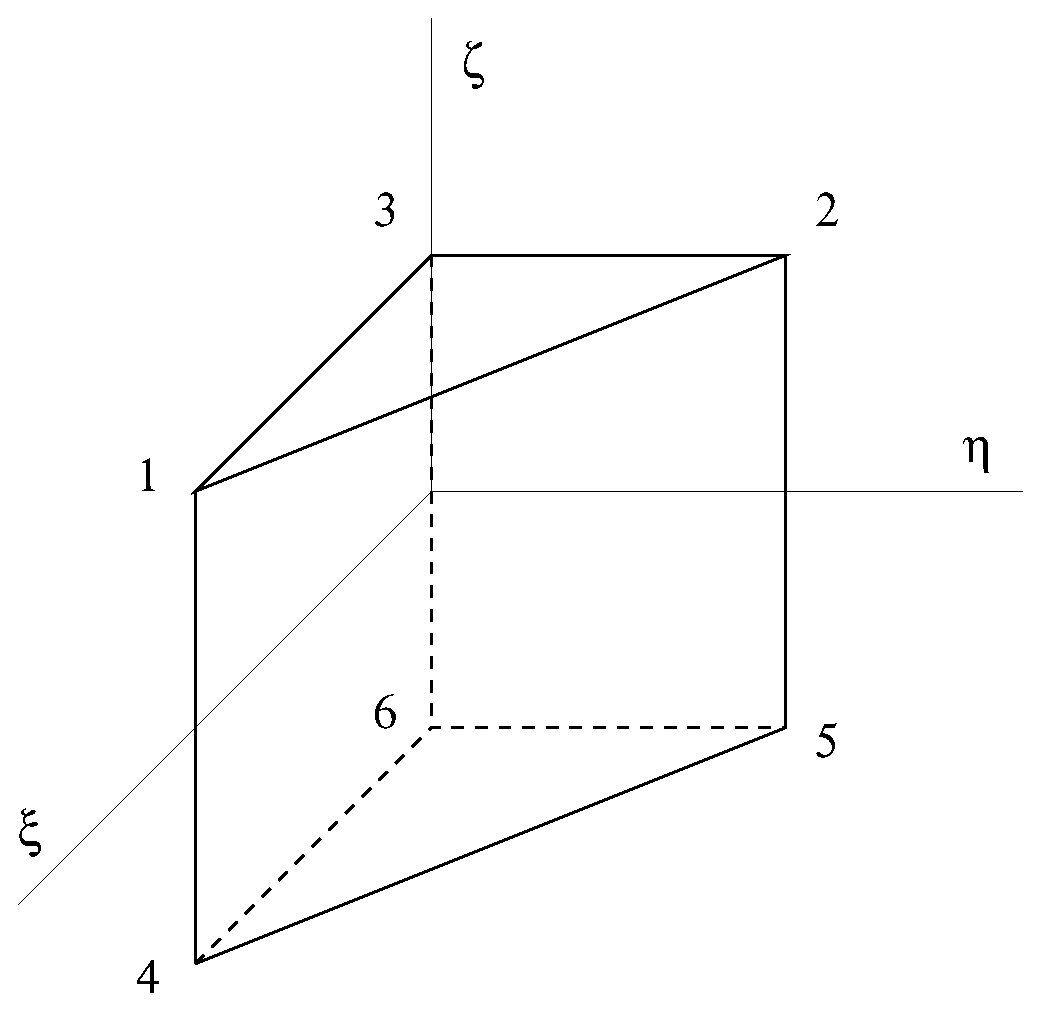
\includegraphics[width=80mm]{FIG/linwedge.eps}
\end{center}
\end{figure}
Partial derivatives with respect to $\xi$ have form
\begin{eqnarray}
\label{bflinweddx1}
\ppd{N_1^{(1)}}{\xi} &=& \del{1}{2} (1 + \zeta)\ ,
\\ \label{bflinweddx2}
\ppd{N_2^{(1)}}{\xi} &=& 0\ ,
\\ \label{bflinweddx3}
\ppd{N_3^{(1)}}{\xi} &=& - \del{1}{2} (1 + \zeta)\ ,
\\ \label{bflinweddx4}
\ppd{N_4^{(1)}}{\xi} &=& \del{1}{2} (1 - \zeta)\ ,
\\ \label{bflinweddx5}
\ppd{N_5^{(1)}}{\xi} &=& 0\ ,
\\ \label{bflinweddx6}
\ppd{N_6^{(1)}}{\xi} &=& - \del{1}{2} (1 - \zeta)\ ,
\end{eqnarray}
Partial derivatives with respect to $\eta$ have form
\begin{eqnarray}
\label{bflinweddy1}
\ppd{N_1^{(1)}}{\eta} &=& 0\ ,
\\ \label{bflinweddy2}
\ppd{N_2^{(1)}}{\eta} &=& \del{1}{2} (1 + \zeta)\ ,
\\ \label{bflinweddy3}
\ppd{N_3^{(1)}}{\eta} &=& - \del{1}{2} (1 + \zeta)\ ,
\\ \label{bflinweddy4}
\ppd{N_4^{(1)}}{\eta} &=& 0\ ,
\\ \label{bflinweddy5}
\ppd{N_5^{(1)}}{\eta} &=& \del{1}{2} (1 - \zeta)\ ,
\\ \label{bflinweddy6}
\ppd{N_6^{(1)}}{\eta} &=& - \del{1}{2} (1 - \zeta)\ ,
\end{eqnarray}
Partial derivatives with respect to $\zeta$ have form
\begin{eqnarray}
\label{bflinweddz1}
\ppd{N_1^{(1)}}{\zeta} &=& \del{\xi}{2}\ ,
\\ \label{bflinweddz2}
\ppd{N_2^{(1)}}{\zeta} &=& \del{\eta}{2}\ ,
\\ \label{bflinweddz3}
\ppd{N_3^{(1)}}{\zeta} &=& \del{1}{2} (1 - \xi - \eta)\ ,
\\ \label{bflinweddz4}
\ppd{N_4^{(1)}}{\zeta} &=& - \del{\xi}{2}\ ,
\\ \label{bflinweddz5}
\ppd{N_5^{(1)}}{\zeta} &=& - \del{\eta}{2}\ ,
\\ \label{bflinweddz6}
\ppd{N_6^{(1)}}{\zeta} &=& - \del{1}{2} (1 - \xi - \eta)\ ,
\end{eqnarray}

%%%%%%%%%%%%%%%%%%%%%%%%%%%%%%%%%%%%%%%%%%%%%%%%%%%%%%%%%%%%%%%%%%%%%%%%%%%%%
%%%%%%%%%%%%%%%%%%%%%%%%%%%%%%%%%%%%%%%%%%%%%%%%%%%%%%%%%%%%%%%%%%%%%%%%%%%%%%%%%%%%%%%%%%%%%%%%
%%%%%%%%%%%%%%%%%%%%%%%%%%%%%%%%%%%%%%%%%%%%%%%%%%%%%%%%%%%%%%%%%%%%%%%%%%%%%%%%%%%%%%%%%%%%%%%%
%%%%%%%%%%%%%%%%%%%%%%%%%%%%%%%%%%%%%%%%%%%%%%%%%%%%%%%%%%%%%%%%%%%%%%%%%%%%%%%%%%%%%%%%%%%%%%%%
%%%%%%%%%%%%%%%%%%%%%%%%%%%%%%%%%%%%%%%%%%%%%%%%%%%%%%%%%%%%%%%%%%%%%%%%%%%%%%%%%%%%%%%%%%%%%%%%
\section{Quadratic approximation functions defined on wedge elements}
$\xi$, $\eta$ and $\zeta$ are natural coordinates. The functions have form
\begin{eqnarray}
\label{bfquadwedn1}
N_1^{(2)} &=& \xi(\xi-0.5)(1 + \zeta)\zeta\ ,
\\
\label{bfquadwedn2}
N_2^{(2)} &=& \eta(\eta-0.5)(1 + \zeta)\zeta\ ,
\\
\label{bfquadwedn3}
N_3^{(2)} &=& (1 - \xi - \eta)(0.5-\xi-\eta)(1 + \zeta)\zeta\ .
\\
\label{bfquadwedn4}
N_4^{(2)} &=& \xi(\xi-0.5)(\zeta - 1)\zeta\ ,
\\
\label{bfquadwedn5}
N_5^{(2)} &=& \eta(\eta-0.5)(\zeta - 1)\zeta\ ,
\\
\label{bfquadwedn6}
N_6^{(2)} &=& (1 - \xi - \eta)(0.5-\xi-\eta)(\zeta - 1)\zeta\ .
\\
\label{bfquadwedn7}
N_7^{(2)} &=& 2 \xi \eta (1 + \zeta)\ ,
\\
\label{bfquadwedn8}
N_8^{(2)} &=& 2 \eta (1 - \xi - \eta)(1 + \zeta)\ ,
\\
\label{bfquadwedn9}
N_9^{(2)} &=& 2 \xi (1 - \xi - \eta)(1 + \zeta)\ ,
\\
\label{bfquadwedn10}
N_{10}^{(2)} &=& \xi (1 - \zeta^2)\ ,
\\
\label{bfquadwedn11}
N_{11}^{(2)} &=& \eta (1 - \zeta^2)\ ,
\\
\label{bfquadwedn12}
N_{12}^{(2)} &=& (1 - \xi - \eta)(1 - \zeta^2)\ ,
\\
\label{bfquadwedn13}
N_{13}^{(2)} &=& 2 \xi \eta (1 - \zeta)\ ,
\\
\label{bfquadwedn14}
N_{14}^{(2)} &=& 2 \eta (1 - \xi - \eta)(1 - \zeta)\ ,
\\
\label{bfquadwedn15}
N_{15}^{(2)} &=& 2 \xi (1 - \xi - \eta)(1 - \zeta)\ ,
\end{eqnarray}


\begin{figure}
\begin{center}
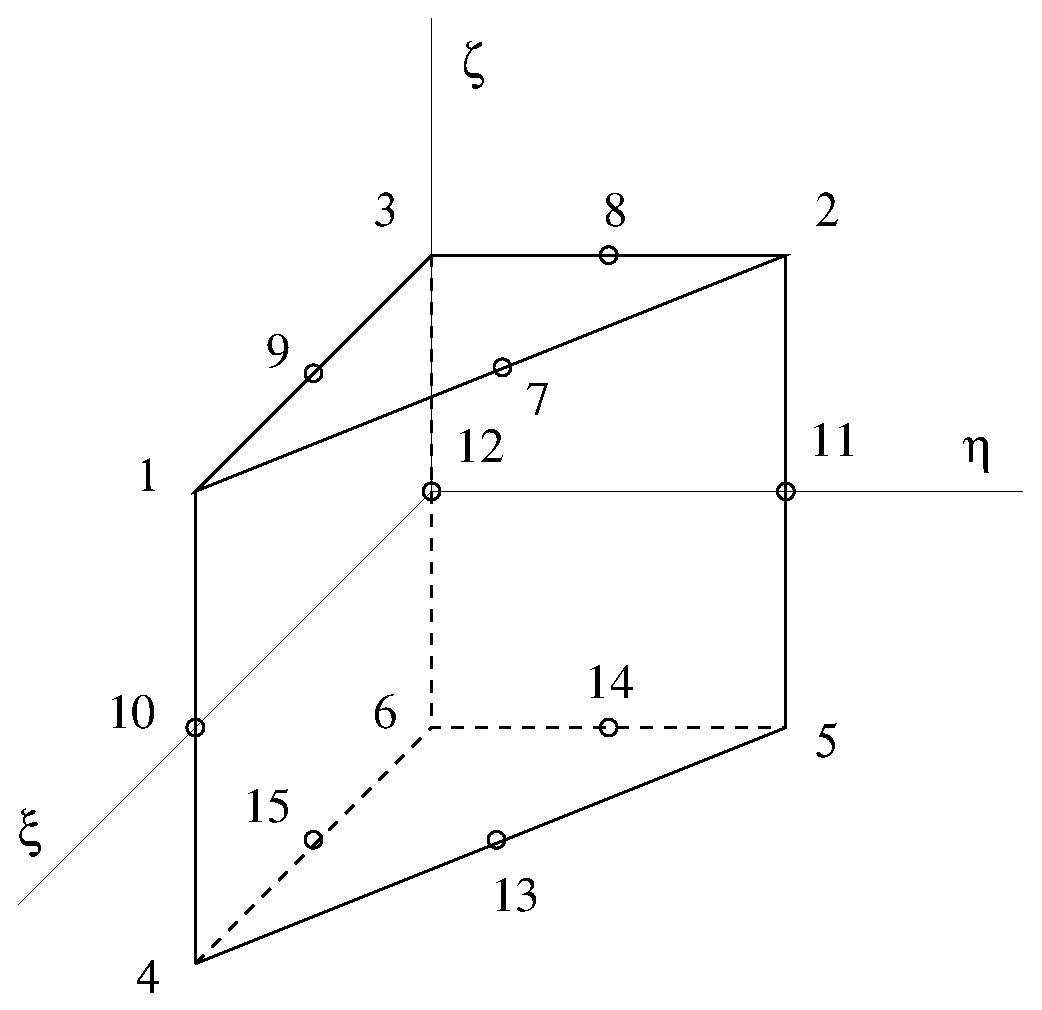
\includegraphics[width=80mm]{FIG/quadwedge.eps}
\end{center}
\end{figure}

Partial derivatives with respect to $\xi$ have form
\begin{eqnarray}
\label{bfquadweddx1}
\ppd{N_1^{(2)}}{\xi} &=& (2 \xi - 0.5) (1 + \zeta)\zeta\ ,
\\
\label{bfquadweddx2}
\ppd{N_2^{(2)}}{\xi} &=& 0\ ,
\\
\label{bfquadweddx3}
\ppd{N_3^{(2)}}{\xi} &=& (2\xi + 2\eta - \del{3}{2})(1 + \zeta)\zeta\ .
\\
\label{bfquadweddx4}
\ppd{N_4^{(2)}}{\xi} &=& (2\xi-0.5)(\zeta - 1)\zeta\ ,
\\
\label{bfquadweddx5}
\ppd{N_5^{(2)}}{\xi} &=& 0\ ,
\\
\label{bfquadweddx6}
\ppd{N_6^{(2)}}{\xi} &=& (2 \xi + 2\eta -\del{3}{2})(\zeta-1)\zeta\ .
\\
\label{bfquadweddx7}
\ppd{N_7^{(2)}}{\xi} &=& 2 \eta (1 + \zeta)\ ,
\\
\label{bfquadweddx8}
\ppd{N_8^{(2)}}{\xi} &=& - 2 \eta (1 + \zeta)\ ,
\\
\label{bfquadweddx9}
\ppd{N_9^{(2)}}{\xi} &=& (2 - 4\xi - 2\eta)(1 + \zeta)\ ,
\\
\label{bfquadweddx10}
\ppd{N_{10}^{(2)}}{\xi} &=& (1 - \zeta^2)\ ,
\\
\label{bfquadweddx11}
\ppd{N_{11}^{(2)}}{\xi} &=& 0\ ,
\\
\label{bfquadweddx12}
\ppd{N_{12}^{(2)}}{\xi} &=& \zeta^2 - 1\ ,
\\
\label{bfquadweddx13}
\ppd{N_{13}^{(2)}}{\xi} &=& 2 \eta (1 - \zeta)\ ,
\\
\label{bfquadweddx14}
\ppd{N_{14}^{(2)}}{\xi} &=& 2 \eta (\zeta - 1)\ ,
\\
\label{bfquadweddx15}
\ppd{N_{15}^{(2)}}{\xi} &=& (2 - 4\xi - 2\eta)(1 - \zeta)\ .
\end{eqnarray}



Partial derivatives with respect to $\eta$ have form
\begin{eqnarray}
\label{bfquadweddy1}
\ppd{N_1^{(2)}}{\eta} &=& 0\ ,
\\
\label{bfquadweddy2}
\ppd{N_2^{(2)}}{\eta} &=& (2\eta-0.5)(1 + \zeta)\zeta\ ,
\\
\label{bfquadweddy3}
\ppd{N_3^{(2)}}{\eta} &=& (2\xi + 2\eta -\del{3}{2})(1 + \zeta)\zeta\ ,
\\
\label{bfquadweddy4}
\ppd{N_4^{(2)}}{\eta} &=& 0\ ,
\\
\label{bfquadweddy5}
\ppd{N_5^{(2)}}{\eta} &=& (2\eta-0.5)(\zeta - 1)\zeta\ ,
\\
\label{bfquadweddy6}
\ppd{N_6^{(2)}}{\eta} &=& (2\xi + 2\eta - \del{3}{2})(\zeta - 1)\zeta\ .
\\
\label{bfquadweddy7}
\ppd{N_7^{(2)}}{\eta} &=& 2 \xi (1 + \zeta)\ ,
\\
\label{bfquadweddy8}
\ppd{N_8^{(2)}}{\eta} &=& (2 - 2\xi - 4\eta)(1 + \zeta)\ ,
\\
\label{bfquadweddy9}
\ppd{N_9^{(2)}}{\eta} &=& -2 \xi (1 + \zeta)\ ,
\\
\label{bfquadweddy10}
\ppd{N_{10}^{(2)}}{\eta} &=& 0\ ,
\\
\label{bfquadweddy11}
\ppd{N_{11}^{(2)}}{\eta} &=& 1 - \zeta^2\ ,
\\
\label{bfquadweddy12}
\ppd{N_{12}^{(2)}}{\eta} &=& \zeta^2 - 1\ ,
\\
\label{bfquadweddy13}
\ppd{N_{13}^{(2)}}{\eta} &=& 2 \xi (1 - \zeta)\ ,
\\
\label{bfquadweddy14}
\ppd{N_{14}^{(2)}}{\eta} &=& (2 - 2\xi - 4\eta)(1 - \zeta)\ ,
\\
\label{bfquadweddy15}
\ppd{N_{15}^{(2)}}{\eta} &=& 2 \xi (\zeta - 1)\ ,
\end{eqnarray}


Partial derivatives with respect to $\zeta$ have form
\begin{eqnarray}
\label{bfquadweddz1}
\ppd{N_1^{(2)}}{\zeta} &=& \xi(\xi-0.5)(1 + 2\zeta)\ ,
\\
\label{bfquadweddz2}
\ppd{N_2^{(2)}}{\zeta} &=& \eta(\eta-0.5)(1 + 2\zeta)\ ,
\\
\label{bfquadweddz3}
\ppd{N_3^{(2)}}{\zeta} &=& (1 - \xi - \eta)(0.5-\xi-\eta)(1 + 2\zeta)\ .
\\
\label{bfquadweddz4}
\ppd{N_4^{(2)}}{\zeta} &=& \xi(\xi-0.5)(2\zeta - 1)\ ,
\\
\label{bfquadweddz5}
\ppd{N_5^{(2)}}{\zeta} &=& \eta(\eta-0.5)(2\zeta - 1)\ ,
\\
\label{bfquadweddz6}
\ppd{N_6^{(2)}}{\zeta} &=& (1 - \xi - \eta)(0.5-\xi-\eta)(2\zeta - 1)\ .
\\
\label{bfquadweddz7}
\ppd{N_7^{(2)}}{\zeta} &=& 2 \xi \eta\ ,
\\
\label{bfquadweddz8}
\ppd{N_8^{(2)}}{\zeta} &=& 2 \eta (1 - \xi - \eta)\ ,
\\
\label{bfquadweddz9}
\ppd{N_9^{(2)}}{\zeta} &=& 2 \xi (1 - \xi - \eta)\ ,
\\
\label{bfquadweddz10}
\ppd{N_{10}^{(2)}}{\zeta} &=& -2 \xi \zeta\ ,
\\
\label{bfquadweddz11}
\ppd{N_{11}^{(2)}}{\zeta} &=& -2 \eta \zeta\ ,
\\
\label{bfquadweddz12}
\ppd{N_{12}^{(2)}}{\zeta} &=& -2 \zeta (1 - \xi - \eta)\ ,
\\
\label{bfquadweddz13}
\ppd{N_{13}^{(2)}}{\zeta} &=& -2 \xi \eta \ ,
\\
\label{bfquadweddz14}
\ppd{N_{14}^{(2)}}{\zeta} &=& -2 \eta (1 - \xi - \eta)\ ,
\\
\label{bfquadweddz15}
\ppd{N_{15}^{(2)}}{\zeta} &=& -2 \xi (1 - \xi - \eta)\ ,
\end{eqnarray}

%%%%%%%%%%%%%%%%%%%%%%%%%%%%%%%%%%%%%%%%%%%%%%%%%%%%%%%%%%%%%%%%%%%%
%%%%%%%%%%%%%%%%%%%%%%%%%%%%%%%%%%%%%%%%%%%%%%%%%%%%%%%%%%%%%%%%%%%%
%%%%%%%%%%%%%%%%%%%%%%%%%%%%%%%%%%%%%%%%%%%%%%%%%%%%%%%%%%%%%%%%%%%%
%%%%%%%%%%%%%%%%%%%%%%%%%%%%%%%%%%%%%%%%%%%%%%%%%%%%%%%%%%%%%%%%%%%%

%%%%%%%%%%%%%%%%%%%%%%%%%%%%%%%%%%%%%%%%%%%%%%%%%%%%%%%%%%%%%%%%%%%%%%%%%%%%%%%%%%%%%%%%%%%%%%%%
%%%%%%%%%%%%%%%%%%%%%%%%%%%%%%%%%%%%%%%%%%%%%%%%%%%%%%%%%%%%%%%%%%%%%%%%%%%%%%%%%%%%%%%%%%%%%%%%
%%%%%%%%%%%%%%%%%%%%%%%%%%%%%%%%%%%%%%%%%%%%%%%%%%%%%%%%%%%%%%%%%%%%%%%%%%%%%%%%%%%%%%%%%%%%%%%%
%%%%%%%%%%%%%%%%%%%%%%%%%%%%%%%%%%%%%%%%%%%%%%%%%%%%%%%%%%%%%%%%%%%%%%%%%%%%%%%%%%%%%%%%%%%%%%%%
\section{Transformation of derivatives}

\subsection{Transformation of derivatives in 2D}

Let function $f$ depends on two variables $x$ and $y$. Let following
relations hold:
\begin{eqnarray}
x(\xi,\eta) &=& \sum_{i=1}^{n} N_i(\xi,\eta) x_i\ ,
\\
y(\xi,\eta) &=& \sum_{i=1}^{n} N_i(\xi,\eta) y_i\ .
\end{eqnarray}
Then function $f$ can be expressed as $f(x,y)=f(x(\xi,\eta),y(\xi,\eta))=f(\xi,\eta)$. The first partial
derivatives of the function $f$ with respect to variables $\xi$ and $\eta$ have form
\begin{eqnarray}
\ppd{f}{\xi} &=& \ppd{f}{x}\ppd{x}{\xi} + \ppd{f}{y}\ppd{y}{\xi}\ ,
\\
\ppd{f}{\eta} &=& \ppd{f}{x}\ppd{x}{\eta} + \ppd{f}{y}\ppd{y}{\eta}\ .
\end{eqnarray}
Previous relations can be rewritten as
\begin{equation}
\left(\begin{array}{cc}
\ppd{x}{\xi} & \ppd{y}{\xi}
\\
\ppd{x}{\eta} & \ppd{y}{\eta}
\end{array}\right)
\left(\begin{array}{c}
\ppd{f}{x}
\\
\ppd{f}{y}
\end{array}\right)
=
\left(\begin{array}{c}
\ppd{f}{\xi}
\\
\ppd{f}{\eta}
\end{array}\right)\ .
\end{equation}
Solution of previous system can be expressed in the form
\begin{eqnarray}
\ppd{f}{x} &=& \del{1}{J}\left(\ppd{f}{\xi}\ppd{y}{\eta} - \ppd{f}{\eta}\ppd{y}{\xi}\right)\ ,
\\
\ppd{f}{y} &=& \del{1}{J}\left(\ppd{f}{\eta}\ppd{x}{\xi} - \ppd{f}{\xi}\ppd{x}{\eta}\right)\ ,
\end{eqnarray}
where $J$ denotes Jacobian and has form
\begin{equation}
J = \ppd{x}{\xi}\ppd{y}{\eta} - \ppd{x}{\eta}\ppd{y}{\xi}\ .
\end{equation}
Let the function $f$ is approximated by $m$ functions
\begin{equation}
f(\xi,\eta) = \sum_{j=1}^{m} M_j(\xi,\eta) f_j\ .
\end{equation}
The first partial derivatives with respect to variables $x$ and $y$ are
\begin{eqnarray}
\ppd{f}{x} &=& \del{1}{J}\left(\sum_{j=1}^{m} \ppd{M_j}{\xi} f_j  \sum_{i=1}^{n} \ppd{N_i}{\eta} y_i -
\sum_{j=1}^{m} \ppd{M_j}{\eta} f_j  \sum_{i=1}^{n} \ppd{N_i}{\xi} y_i\right)\ ,
\\
\ppd{f}{y} &=& \del{1}{J}\left(\sum_{j=1}^{m} \ppd{M_j}{\eta} f_j  \sum_{i=1}^{n} \ppd{N_i}{\xi} x_i -
\sum_{j=1}^{m} \ppd{M_j}{\xi} f_j  \sum_{i=1}^{n} \ppd{N_i}{\eta} x_i\right)\ ,
\end{eqnarray}



%%%%%%%%%%%%%%%%%%%%%%%%%%%%%%%%%%%%%%%%%%%%%%%%%%%%%%%%%%%%%%%%%%%%
%%%%%%%%%%%%%%%%%%%%%%%%%%%%%%%%%%%%%%%%%%%%%%%%%%%%%%%%%%%%%%%%%%%%
%%%%%%%%%%%%%%%%%%%%%%%%%%%%%%%%%%%%%%%%%%%%%%%%%%%%%%%%%%%%%%%%%%%%
%%%%%%%%%%%%%%%%%%%%%%%%%%%%%%%%%%%%%%%%%%%%%%%%%%%%%%%%%%%%%%%%%%%%
\subsection{Transformation of derivatives in 3D}

Let function $f$ depends on three variables $x$,$y$ and $z$. Let following
relations hold:
\begin{eqnarray}
x(\xi,\eta,\zeta) &=& \sum_{i=1}^{n} N_i(\xi,\eta,\zeta) x_i\ ,
\\
y(\xi,\eta,\zeta) &=& \sum_{i=1}^{n} N_i(\xi,\eta,\zeta) y_i\ ,
\\
z(\xi,\eta,\zeta) &=& \sum_{i=1}^{n} N_i(\xi,\eta,\zeta) z_i\ .
\end{eqnarray}
Then function $f$ can be expressed as
$f(x,y,z)=f(x(\xi,\eta,\zeta),y(\xi,\eta,\zeta),z(\xi,\eta,\zeta))=f(\xi,\eta,\zeta)$. The first partial
derivatives of the function $f$ with respect to variables $\xi$,$\eta$ and $\zeta$ have form
\begin{eqnarray}
\ppd{f}{\xi} &=& \ppd{f}{x}\ppd{x}{\xi} + \ppd{f}{y}\ppd{y}{\xi} + \ppd{f}{z}\ppd{z}{\xi}\ ,
\\
\ppd{f}{\eta} &=& \ppd{f}{x}\ppd{x}{\eta} + \ppd{f}{y}\ppd{y}{\eta} + \ppd{f}{z}\ppd{z}{\eta}\ ,
\\
\ppd{f}{\zeta} &=& \ppd{f}{x}\ppd{x}{\zeta} + \ppd{f}{y}\ppd{y}{\zeta} + \ppd{f}{z}\ppd{z}{\zeta}\ .
\end{eqnarray}
Previous relations can be rewritten as
\begin{equation}
\left(\begin{array}{ccc}
\ppd{x}{\xi} & \ppd{y}{\xi} & \ppd{z}{\xi}
\\
\ppd{x}{\eta} & \ppd{y}{\eta} & \ppd{z}{\eta}
\\
\ppd{x}{\zeta} & \ppd{y}{\zeta} & \ppd{z}{\zeta}
\end{array}\right)
\left(\begin{array}{c}
\ppd{f}{x}
\\
\ppd{f}{y}
\\
\ppd{f}{z}
\end{array}\right)
=
\left(\begin{array}{c}
\ppd{f}{\xi}
\\
\ppd{f}{\eta}
\\
\ppd{f}{\zeta}
\end{array}\right)\ .
\end{equation}
Solution of previous system can be expressed in the form
\begin{eqnarray}
\ppd{f}{x} &=& \del{1}{J}\left(
\ppd{f}{\xi}\ppd{y}{\eta}\ppd{z}{\zeta} + \ppd{f}{\zeta}\ppd{y}{\xi}\ppd{z}{\eta} +
\ppd{f}{\eta}\ppd{y}{\zeta}\ppd{z}{\xi} -\right.
\\
&-& \left.\ppd{f}{\zeta}\ppd{y}{\eta}\ppd{z}{\xi} -
\ppd{f}{\xi}\ppd{y}{\zeta}\ppd{z}{\eta} - \ppd{f}{\eta}\ppd{y}{\xi}\ppd{z}{\zeta}
\right)\ ,
\\
\ppd{f}{y} &=& \del{1}{J}\left(
\ppd{f}{\eta}\ppd{x}{\xi}\ppd{z}{\zeta} + \ppd{f}{\xi}\ppd{x}{\zeta}\ppd{z}{\eta} +
\ppd{f}{\zeta}\ppd{x}{\eta}\ppd{z}{\xi} -\right.
\\
&-& \left.\ppd{f}{\eta}\ppd{x}{\zeta}\ppd{z}{\xi} -
\ppd{f}{\zeta}\ppd{x}{\xi}\ppd{z}{\eta} - \ppd{f}{\xi}\ppd{x}{\eta}\ppd{z}{\zeta}
\right)\ ,
\\
\ppd{f}{z} &=& \del{1}{J}\left(
\ppd{f}{\zeta}\ppd{x}{\xi}\ppd{y}{\eta} + \ppd{f}{\eta}\ppd{x}{\zeta}\ppd{y}{\xi} +
\ppd{f}{\xi}\ppd{x}{\eta}\ppd{y}{\zeta} -\right.
\\
&-& \left.\ppd{f}{\xi}\ppd{x}{\zeta}\ppd{y}{\eta} -
\ppd{f}{\eta}\ppd{x}{\xi}\ppd{y}{\zeta} - \ppd{f}{\zeta}\ppd{x}{\eta}\ppd{y}{\xi}
\right)\ ,
\end{eqnarray}
where $J$ denotes Jacobian and has form
\begin{equation}
J = 
\ppd{x}{\xi}\ppd{y}{\eta}\ppd{z}{\zeta} + \ppd{x}{\zeta}\ppd{y}{\xi}\ppd{z}{\eta} +
\ppd{x}{\eta}\ppd{y}{\zeta}\ppd{z}{\xi} - \ppd{x}{\zeta}\ppd{y}{\eta}\ppd{z}{\xi} -
\ppd{x}{\xi}\ppd{y}{\zeta}\ppd{z}{\eta} - \ppd{x}{\eta}\ppd{y}{\xi}\ppd{z}{\zeta}\ .
\end{equation}
Let the function $f$ is approximated by $m$ functions
\begin{equation}
f(\xi,\eta,\zeta) = \sum_{j=1}^{m} M_j(\xi,\eta,\zeta) f_j\ .
\end{equation}
The first partial derivatives with respect to variables $x$,$y$ and $z$ are
\begin{eqnarray}\nonumber
\ppd{f}{x} &=& \del{1}{J}\left(
\sum_{j=1}^{m}\ppd{M_j}{\xi}f_j \sum_{i=1}^{n}\ppd{N_i}{\eta}y_i \sum_{i=1}^{n}\ppd{N_i}{\zeta}z_i +
\sum_{j=1}^{m}\ppd{M_j}{\zeta}f_j \sum_{i=1}^{n}\ppd{N_i}{\xi}y_i \sum_{i=1}^{n}\ppd{N_i}{\eta}z_i +\right.
\\[2mm] \nonumber &+&
\sum_{j=1}^{m}\ppd{M_j}{\eta}f_j \sum_{i=1}^{n}\ppd{N_i}{\zeta}y_i \sum_{i=1}^{n}\ppd{N_i}{\xi}z_i -
\sum_{j=1}^{m}\ppd{M_j}{\zeta}f_j \sum_{i=1}^{n}\ppd{N_i}{\eta}y_i \sum_{i=1}^{n}\ppd{N_i}{\xi}z_i -
\\ &-& \left.
\sum_{j=1}^{m}\ppd{M_j}{\xi}f_j \sum_{i=1}^{n}\ppd{N_i}{\zeta}y_i \sum_{i=1}^{n}\ppd{N_i}{\eta}z_i -
\sum_{j=1}^{m}\ppd{M_j}{\eta}f_j \sum_{i=1}^{n}\ppd{N_i}{\xi}y_i \sum_{i=1}^{n}\ppd{N_i}{\zeta}z_i
\right)\ ,
\\ \nonumber
\ppd{f}{y} &=& \del{1}{J}\left(
\sum_{j=1}^{m}\ppd{M_j}{\eta}f_j \sum_{i=1}^{n}\ppd{N_i}{\xi}x_i \sum_{i=1}^{n}\ppd{N_i}{\zeta}z_i +
\sum_{j=1}^{m}\ppd{M_j}{\xi}f_j \sum_{i=1}^{n}\ppd{N_i}{\zeta}x_i \sum_{i=1}^{n}\ppd{N_i}{\eta}z_i +\right.
\\ &+& \nonumber
\sum_{j=1}^{m}\ppd{M_j}{\zeta}f_j \sum_{i=1}^{n}\ppd{N_i}{\eta}x_i \sum_{i=1}^{n}\ppd{N_i}{\xi}z_i -
\sum_{j=1}^{m}\ppd{M_j}{\eta}f_j \sum_{i=1}^{n}\ppd{N_i}{\zeta}x_i \sum_{i=1}^{n}\ppd{N_i}{\xi}z_i -
\\ &-& \left.
\sum_{j=1}^{m}\ppd{M_j}{\zeta}f_j \sum_{i=1}^{n}\ppd{N_i}{\xi}x_i \sum_{i=1}^{n}\ppd{N_i}{\eta}z_i -
\sum_{j=1}^{m}\ppd{M_j}{\xi}f_j \sum_{i=1}^{n}\ppd{N_i}{\eta}x_i \sum_{i=1}^{n}\ppd{N_i}{\zeta}z_i
\right)\ ,
\\ \nonumber
\ppd{f}{z} &=& \del{1}{J}\left(
\sum_{j=1}^{m}\ppd{f}{\zeta}f_j \sum_{i=1}^{n}\ppd{N_i}{\xi}x_i \sum_{i=1}^{n}\ppd{N_i}{\eta}y_i +
\sum_{j=1}^{m}\ppd{f}{\eta}f_j \sum_{i=1}^{n}\ppd{N_i}{\zeta}x_i \sum_{i=1}^{n}\ppd{N_i}{\xi}y_i +\right.
\\ &+& \nonumber
\sum_{j=1}^{m}\ppd{f}{\xi}f_j \sum_{i=1}^{n}\ppd{N_i}{\eta}x_i \sum_{i=1}^{n}\ppd{N_i}{\zeta}y_i -
\sum_{j=1}^{m}\ppd{f}{\xi}f_j \sum_{i=1}^{n}\ppd{N_i}{\zeta}x_i \sum_{i=1}^{n}\ppd{N_i}{\eta}y_i -
\\ &-& \left.
\sum_{j=1}^{m}\ppd{f}{\eta}f_j \sum_{i=1}^{n}\ppd{N_i}{\xi}x_i \sum_{i=1}^{n}\ppd{N_i}{\zeta}y_i -
\sum_{j=1}^{m}\ppd{f}{\zeta}f_j \sum_{i=1}^{n}\ppd{N_i}{\eta}x_i \sum_{i=1}^{n}\ppd{N_i}{\xi}y_i
\right)\ ,
\end{eqnarray}
%%%%%%%%%%%%%%%%%%%%%%%%%%%%%%%%%%%%%%%%%%%%%%%%%%%%%%%%%%%%%%%%%%%%
%%%%%%%%%%%%%%%%%%%%%%%%%%%%%%%%%%%%%%%%%%%%%%%%%%%%%%%%%%%%%%%%%%%%
%%%%%%%%%%%%%%%%%%%%%%%%%%%%%%%%%%%%%%%%%%%%%%%%%%%%%%%%%%%%%%%%%%%%
%%%%%%%%%%%%%%%%%%%%%%%%%%%%%%%%%%%%%%%%%%%%%%%%%%%%%%%%%%%%%%%%%%%%
